\documentclass[10pt,a4paper,oneside]{article}

% This first part of the file is called the PREAMBLE. It includes
% customizations and command definitions. The preamble is everything
% between \documentclass and \begin{document}.

\usepackage[margin=1in]{geometry}  % set the margins to 1in on all sides
\usepackage{graphicx}              % to include figures
\usepackage{amsmath}               % great math stuff
\usepackage{amsfonts}              % for blackboard bold, etc
\usepackage{amsthm}                % better theorem environments
\usepackage[english]{babel}
\usepackage[square, numbers]{natbib}
\usepackage[T1]{fontenc}
\usepackage[utf8]{inputenc}
\usepackage{lmodern}
\usepackage{amssymb}
\usepackage{authoraftertitle}
\usepackage{hyperref}
\usepackage{multicol}
\usepackage{caption}
\usepackage{subcaption}
\usepackage{placeins}
\usepackage{setspace}
\usepackage{wrapfig}

%\onehalfspace
\singlespace

% Author
\author{Ondrej Škopek\\
Faculty of Mathematics and Physics\\
Charles University in Prague\\
\texttt{\href{mailto:oskopek@matfyz.cz}{oskopek@matfyz.cz}}}

\title{Individual Software Project specification -- TransportEditor}

%\date{3. mája 2015}
\date{\today}

% hyperref

\hypersetup{
    bookmarks=true,         % show bookmarks bar?
    unicode=true,          % non-Latin characters in Acrobat’s bookmarks
    pdftoolbar=true,        % show Acrobat’s toolbar?
    pdfmenubar=true,        % show Acrobat’s menu?
    pdffitwindow=true,     % window fit to page when opened
    pdfstartview={FitV},    % fits the width of the page to the window
    pdftitle={\MyTitle},    % title
    pdfauthor={\MyAuthor},     % author
    pdfsubject={\MyTitle},   % subject of the document
    pdfcreator={\MyAuthor},   % creator of the document
    pdfproducer={\MyAuthor}, % producer of the document
    pdfkeywords={software} {project} {planning} {automated planning} {java} {javafx} {ipc} {icaps} {transport} {transport domain}, % list of keywords
    pdfnewwindow=true,      % links in new PDF window
    colorlinks=false,       % false: boxed links; true: colored links
    linkcolor=red,          % color of internal links (change box color with linkbordercolor)
    citecolor=green,        % color of links to bibliography
    filecolor=magenta,      % color of file links
    urlcolor=cyan,           % color of external links
}


% various theorems, numbered by section

\newtheorem{thm}{Theorem}[section]
\newtheorem{lem}[thm]{Lemma}
\newtheorem{obsv}[thm]{Observation}
\newtheorem{cor}[thm]{Corollary}
\newtheorem{conj}[thm]{Conjecture}

\DeclareMathOperator{\id}{id}

\newcommand{\TODO}[1]{{\textbf{TODO:} #1}} % for TODOs
\newcommand{\comment}[1]{} % for comments

\newcommand{\dist}{\text{dist}} % distance function
\newcommand{\bd}[1]{\mathbf{#1}} % for bolding symbols 
\newcommand{\RR}{\mathbb{R}}      % for Real numbers
\newcommand{\ZZ}{\mathbb{Z}}      % for Integers
\newcommand{\col}[1]{\left[\begin{matrix} #1 \end{matrix} \right]}
\newcommand{\comb}[2]{\binom{#1^2 + #2^2}{#1+#2}}
\newcommand{\pname}{TransportEditor} % project name (or code name)

\begin{document}
\maketitle











\section{Basic information}

\pname{} aims to be a problem editor and plan visualizer for the Transport domain from the International Planning Competition 2008.
The goal is to create an intuitive GUI desktop application for making quick changes and re-planning, but also designing a new problem dataset from scratch. \pname{} will help researchers working on this domain fine-tune their planners; they can visualize the various corner cases their planner fails to handle, step through the generated plan and find the points where their approach fails.
A secondary motivation is to be able to test approaches for creating plans for the domain as part of our future bachelor thesis.

\subsection{The Transport planning domain} \label{domain-info}

Transport is a domain designed originally for the International Planning Competition (IPC, part of the International Conference on Automated Planning and Scheduling ICAPS).
Originally, Transport appeared at \href{http://icaps-conference.org/ipc2008/deterministic/Domains.html}{IPC-6 2008}.
Since then, it has been used in every IPC, specifically \href{http://www.plg.inf.uc3m.es/ipc2011-deterministic/}{IPC-7 2011}
and \href{https://helios.hud.ac.uk/scommv/IPC-14/}{IPC-8 2014}.

There are two basic formulations of the Transport domain family (i.e. two ``similar Transport domains''):
\begin{itemize}
\item \verb+transport-strips+ -- the classical, sequential Transport domain. See section \ref{transport-strips} for details.
\item \verb+transport-numeric+ -- the numerical Transport domain. See section \ref{transport-numeric} for details.
\end{itemize}

Both of these formulations have been used interchangeably in various competition tracks.
The following is an overview of the distinct datasets, their associated IPC competition, track at the competition and the formulation used (descriptions of the tracks in hyperlinks):

\begin{center}
\begin{tabular}{c|c|c|c}
\textbf{Dataset name} & \textbf{Competition} & \textbf{Track} & \textbf{Formulation} \\ 
\hline
\hline
netben-opt-6 & IPC-6 & \href{http://icaps-conference.org/ipc2008/deterministic/NetBenefitOptimization.html}{Net-benefit: optimal} & Numeric \\ 
seq-opt-6 & IPC-6 & \href{http://icaps-conference.org/ipc2008/deterministic/SequentialSatisficing.html}{Sequential: satisficing} & STRIPS \\ 
seq-sat-6 & IPC-6 & \href{http://icaps-conference.org/ipc2008/deterministic/SequentialOptimization.html}{Sequential: optimal} & STRIPS \\ 
tempo-sat-6 & IPC-6 & \href{http://icaps-conference.org/ipc2008/deterministic/TemporalSatisficing.html}{Temporal: satisficing} & Numeric \\ 
\hline
seq-agl-8 & IPC-8 & \href{https://helios.hud.ac.uk/scommv/IPC-14/seqagi.html}{Sequential: agile} & STRIPS \\ 
seq-mco-8 & IPC-8 & \href{https://helios.hud.ac.uk/scommv/IPC-14/seqmulti.html}{Sequential: multi-core} & STRIPS \\ 
seq-opt-8 & IPC-8 & \href{https://helios.hud.ac.uk/scommv/IPC-14/seqopt.html}{Sequential: optimal} & STRIPS \\ 
seq-sat-8 & IPC-8 & \href{https://helios.hud.ac.uk/scommv/IPC-14/seqsat.html}{Sequential: satisficing} & STRIPS \\ 
\end{tabular} 
\end{center}

Short descriptions of the various tracks and subtracks can be found in the rule pages of
\href{https://helios.hud.ac.uk/scommv/IPC-14/rules.html}{IPC-6}
and the  \href{http://icaps-conference.org/ipc2008/deterministic/CompetitionRules.html}{rule page of IPC-8}.

Unfortunately, we weren't able to acquire the datasets for IPC-7, as the \href{http://www.plg.inf.uc3m.es/ipc2011-deterministic/Domains.html}{Subversion repository} that promises to contain them is unavailable.

As a bonus, \pname{} supports custom domains based on the Transport domain family. Users can create new Transport-like domains that have any subset of constraints/features of the two basic formulations. Only subsets in which individual constraints are not in conflict with each other are allowed.

\subsection{Transport STRIPS formulation description}\label{transport-strips}

The STRIPS version of Transport is a logistics domain -- vehicles with limited capacities drive around on a (generally asymmetric) positively-weighted oriented graph, picking up and dropping packages along the way. Picking up or dropping a package costs 1, driving along a road costs depending on the edge weight. All packages have a size of 1. The general aim is to minimize the total cost, while delivering all packages to their destination.

\subsection{Transport Numeric formulation description}\label{transport-numeric}

The numerical version of Transport is very similar to the STRIPS version, see section \ref{transport-strips}. The key differences are:
\begin{itemize}
\item Package sizes can now be any positive number.
\item The concept of fuel -- every vehicle has a maximum fuel level, current fuel level, and all roads have a fuel demand (generally different than the length of the road). A vehicle can refuel if there is a petrol station at the given location. Refuelling always fills the vehicle's tank to the max.
\item The introduction of time:
\begin{itemize}
\item The duration of driving along a road is equal to it's length.
\item The duration of picking a package up or dropping it off is equal to 1.
\item The duration of refuelling is equal to 10.
\item A vehicle cannot pick up or drop packages concurrently -- it always handles packages one at a time.
\item A vehicle cannot do other actions during driving to another location (it is essentially placed ``off the graph'' for the duration of driving).
\end{itemize}
\item The cost function is removed (we now minimize the total duration of a plan).
\end{itemize}


















\section{Feature requirements}

In this section, we present the basic functionality requirements for \pname{}.

\subsection{Functionality overview}

The basic workflow of \pname{} consists of the following user's steps:
\begin{itemize}
\item Select which formulation of the Transport domain they want to work with or create their own variant.
\item Load or create their own problem of the given domain. See section \ref{input-output} for details on the input format.
\item \pname{} draws the given graph as good as it can.
\item Iterate among the following options:
\begin{itemize}
\item Load a planner executable and let \pname{} run the planner on the loaded problem instance for a given time, then load the resulting plan.
\item Load a pre-generated plan.
\item Step through the individual plan actions and let \pname{} visualize them.
The user can go forward and backward in the plan and inspect each step in great detail.
\item Edit the graph: add/remove/edit the location or properties of vehicles, packages, roads, locations and possibly petrol stations.
\item Save the currently generated plan.
\item Save the problem (along with the graph drawing hints).
\item Save the domain (export to a PDDL file).
\end{itemize}
\item Save and close the currently loaded problem. Exit the application or go back to the first step.
\end{itemize}

There are a lot of requirements that arise from the typical workflow above. We will describe them in the next few sections.

\subsection{User interface functionality} \label{ui}

In order for \pname{} to be useful to it's users, it has to have enable a quick and efficient workflow.
The biggest challenge will be to design an intuitive and responsive graphical user interface.
Key parts of the user interface are:
\begin{itemize}
\item A large and not crowded drawing of the road graph, showing only the most relevant information, possibly letting the user display details on-demand.
\item A clear and concise list of actions in the plan the user wants to visualize.
\item A panel of tools to edit the problem and graph with.
\end{itemize}

We will describe these three in detail in the following sections. For an image that aims to capture the formulated requirements, see section \ref{ui-layout}.

\subsubsection{Graph visualization} \label{graphviz}

\begin{wrapfigure}{r}{0.5\textwidth}
        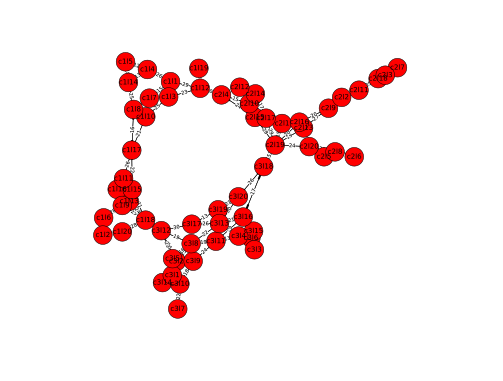
\includegraphics[width=0.6\textwidth]{../data/img/pdf/seq-sat-6-p30}
        \caption{seq-sat-6-p30 prototype graph drawing. Drawn using the
         \href{http://emr.cs.iit.edu/~reingold/force-directed.pdf}{Fruchterman \& Reingold algorithm}
         with the help of  \href{https://networkx.github.io/}{NetworkX}.}
        \label{fig:graph}
\end{wrapfigure}

Above all, the graph should be reasonably well arranged and drawn. However, drawing an arbitrary graph is considered a hard problem on it's own.
We will focus on implementing a reasonable graph drawing algorithm and let the user make manual drag-and-drop style changes on top of the graph drawing we produce.

A more specific property of the Transport domain graphs is that they have quite a lot of data on the edges (roads) and vertexes (locations) -- road lengths, fuel demands, location names and petrol station, package and vehicle current locations.
Clearly, this cannot fit on the graph drawing at once -- we will have to do selective drawing of the information in order
not to crowd the graph.
Popping up overlays on user mouse-over
or a graph legend where the user can select what info to currently show are just a few options.

To highlight the need for selective drawing of information, observe the following image on the right (figure \ref{fig:graph}) -- a graph drawing of the p30 problem from the seq-sat-6 dataset.

Another important feature is symbolic visualization of individual actions in the plan.
There are only 3-4 actions in the Transport domain family (drive, pick-up, drop and possibly refuel in the numerical formulation).
We need to be able to visualize the selected plan action in the graph to help the user see what is going on in the plan.

\subsubsection{Plan action list} \label{plan-action-list}

An important part of the visualization workflow is the actual planner-generated plan.
The user interface will show a context-aware list of them.

Because plans can be quite long (generally hundreds/thousands of actions),
we cannot show them all at once.
The list will only show the currently selected action, a few actions preceding it and a few upcoming actions.

The graph described in section \ref{graphviz} and the state it represents will change dynamically with the selected action in the list. The user can fluently scroll through the plan actions, continually stepping through the plan either forwards or backwards.
Jumping to a specific action will also be supported.

If users want to view the effect of a small change in the plan, they can choose to edit the current plan action or reorder it (move it up or down).
In the case of temporal domains, they can edit the start time of actions.
A user reordering or editing an action cannot invalidate the plan -- there will be dynamic validation in place, which will disable any changes that make the plan invalid.

The list will also support filtering: the user can choose to view only those actions, which involve a certain subset of planning objects (vehicle, package, road, \ldots) in the given problem.

Above the plan action list, there will be buttons to allow planning or re-planning the current problem using a planner the users choice.
During planning, \pname{} will attempt to show the currently best found plan, if it gets the needed information from the planner.

\subsubsection{Editing tools}

A big feature of \pname{} is editing the domain problems on the fly.
All the graph vertexes will be movable using drag-and-drop (the edges will move along, too).
Details of individual elements on the graph (vehicles, packages, locations, roads) will be editable
on user request.

Additionally, a toolbox will be present. It will enable quick access to buttons for adding/removing locations, roads, vehicles and packages.

To prevent accidental changes to the problem when we just want to test plan generation,
the toolbox will contain a lock feature -- once enabled, no changes to the graph will be allowed.

\subsection{Performance}

The performance requirements of \pname{} cannot be quantified numerically -- the only criterion is, that the application must be sufficiently
responsive to user actions. The implementation specific details on how to achieve this are discussed in the section \ref{used-tech}.

\subsection{Data model re-usability}

The internal data representation has to be reusable and therefore, reasonably decoupled from the rest of the application.
It is very probable that we will want to implement a planner for the Transport domain later on
-- and for that, we can reuse the entire back-end data model that is used to represent the domain problem in memory
and build the planner on top of it.
More details on the specifics of decoupling of individual modules of \pname{} are in section \ref{modules}.

\subsection{Optional features}

A few more optional features, which may or may not be included in the final product:

\begin{itemize}
\item Automatic plan verification -- Upon loading a plan, verify (using VAL) that the plan is valid for the given problem and domain. See section \ref{plan-format} for more information.
\item When a user select a certain subset of planning object to focus on in the plan action list (see section \ref{plan-action-list}), visualize those on the graph (section \ref{graphviz}).
\item Various plan action list visualizations (can be selected based on user preferences):
\begin{itemize}
\item \href{https://en.wikipedia.org/wiki/Gantt_chart}{Gantt chart} -- can clearly visualize changes in planning object properties (f.~e.~vehicle capacity).
\item Partially ordered action graph -- visualizes preconditions and effects of actions clearly, allows the user to see what is ``holding up'' the action.
\item Time-ordered multi-list -- for domains without temporal conditions, is equivalent to the original plan action list. For temporal domains, this visualizes concurrently occurring actions side-by-side -- the user can clearly see the relation between duration intervals of actions.
\end{itemize}
\end{itemize}









\section{Program decomposition}

In this section, we present a basic decomposition of the application from the logical perspective.

\subsection{Modules} \label{modules}

The application will be split up into individual modules.
Modules should be decoupled as much as possible, communicating only through well specified interfaces.
We propose the following modules:

\begin{itemize}
\item View -- representation of the individual UI elements.
\item Controller -- an interfacing module, sitting between the view and model. Serves as a mediator -- updating the view based on model changes, and propagating user actions from the view back into the model.
\item Model -- the back-end data model, an internal problem data representation.
\item Persistence -- handles saving/loading the model and plans for the model to an external data store (f.e.~hard disk).
\end{itemize}

%\subsection{UML diagram of the model}
%
%\TODO Add a UML diagram of the model


\section{Software description}

In this section, we describe the chosen technology and how we aim to fulfil the requirements using it.

\subsection{Used technologies} \label{used-tech}

We have to chosen to implement the application along with the graphical user interface as a
desktop Java 8 program. The main reasons for this choice were portability and our experiences working in Java and it's associated technologies.

The reason for choosing Java 8 as the minimum version is JavaFX 8 -- a successor of JavaFX 2.0, now newly incorporated into
the standard Java Runtime Environment (JRE) and available on all Java Standard Edition (Java SE) versions of the JRE.

The model will use features not specific to JavaFX and therefore be reusable in any standard Java SE 8 and newer program.

We will probably use multiple open-source libraries which will all be specified in the developer documentation (section \ref{docs})
to write cleaner, more expressive code.

The application will be shipped as a ZIP archive, containing an executable JAR file and the user documentation.

\subsubsection{Environment dependencies}

The runtime dependencies that are implied by the previous section are:
\begin{itemize}
\item Java SE, version 8+
\end{itemize}
All other dependencies will be packaged and shipped along with the product.

The development dependencies will be:
\begin{itemize}
\item Java SE, version 8+
\item Maven, version 3+
\end{itemize}

Any hardware dependencies or arising software dependencies will be specified in the user or developer documentation (section \ref{docs}).

\subsection{Proposed user interface layout} \label{ui-layout}

The following image (figure \ref{fig:gui}) aims to be a an abstract draft for the application's user interface.
More details on the specifics of the UI can be found in section \ref{ui}.
\begin{figure}[h]
        \centering
        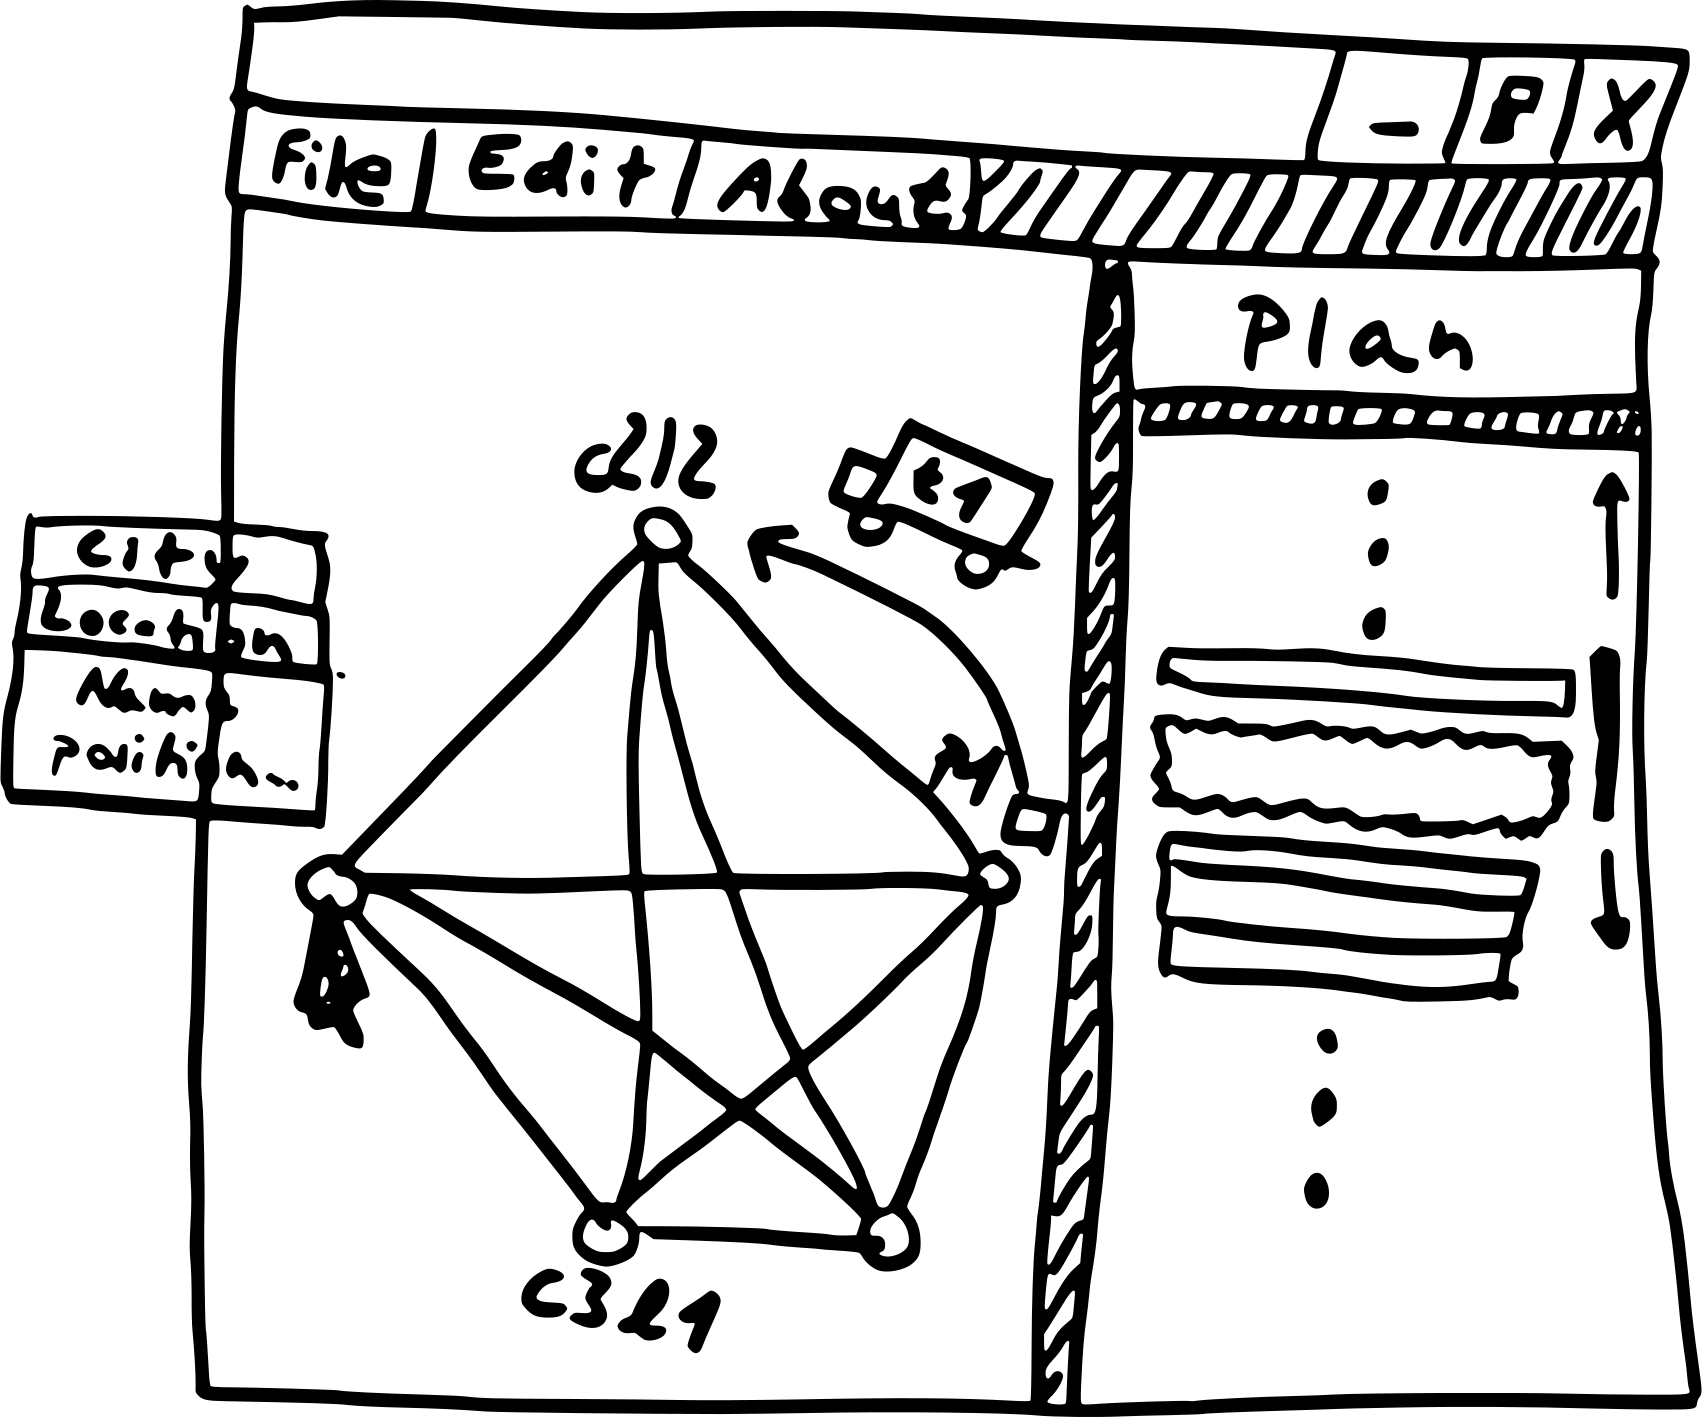
\includegraphics[width=0.73\textwidth]{../data/img/pdf/gui}
        \caption{Abstract GUI prototype}
        \label{fig:gui}
\end{figure}


\subsection{User and developer documentation} \label{docs}

We hope most of the user documentation will be left unread -- the user interface and workflow should be
mostly self-explainable and intuitive.
Nevertheless, we will produce user documentation, involving:
\begin{itemize}
\item A help document accessible from the menu bar inside the application.
\item Helpful hint and validation dialog windows or other pop-up messages. In general, we do not want to let the user do something that is be invalid, rather than notifying him of his error afterwards. Therefore, we disable buttons where appropriate, validate inputs, \ldots
\item A standalone text document, documenting the features, supported data formats, instructions on the installing Java JRE and a demo usage tutorial.
\end{itemize}

The developer documentation consists of in-code comments, Java Doc comments (and a generated HTML page hierarchy using the \verb+javadoc+ tool) and a standalone text file, containing information on:
\begin{itemize}
\item Links to the code repository, issue tracker, continuous integration service, \ldots
\item Getting the code from the code repository.
\item Installing the needed dependencies.
\item Compiling and building the project.
\item Finding their way around the project -- a high-level overview of the project, module content and usage descriptions, \ldots
\end{itemize}






\section{Input \& output format} \label{input-output}

There are two fundamentally different files \pname{} works with: problems and plans.
Problem files contain information on the domain problem (roads, vehicles, packages, locations, \ldots).
Plan files contain a sequence of actions on a specific problem that (if a plan is valid) constitute a plan
for the given problem.

\subsubsection{Domain problem file format}\label{problem-format}

Both rule pages of \href{http://icaps-conference.org/ipc2008/deterministic/CompetitionRules.html}{IPC-6}
and \href{https://helios.hud.ac.uk/scommv/IPC-14/rules.html}{IPC-8}
specify PDDL 3.1 as their official modelling language. Daniel L. Kovacs proposed an updated and corrected BNF (Backus-Naur Form)
\href{https://helios.hud.ac.uk/scommv/IPC-14/repository/kovacs-pddl-3.1-2011.pdf}{definition of PDDL 3.1}.

\pname{} doesn't load the PDDL domain definitions directly -- those are already built-in.
We only read the domain files to check which subset of conditions the user has chosen to model.
See section \ref{domain-info} for more information.
The loaded problem has to be compatible with the loaded domain variant.
\pname{} will make an attempt to read problems which have more information than are needed for the currently modelled domain.

To allow \pname{} to save the positions of vertexes in the graph, we make use of an already used ``unwritten extension' of PDDL':
above every road predicate, there is a comment in the form of \verb+; a,b -> c,d+,
where \verb+a+, \verb+b+, \verb+c+ and \verb+d+ are integers (non-negative whole numbers).
Those numbers correspond to the coordinates of the source \verb+(a,b)+ and destination \verb+(c,d)+ locations of the defined road on the line below. The upper left corner of the drawing corresponds to the \verb+(0,0)+ point. A point with the coordinates \verb+(x,y)+ is \verb+x+ units below and \verb+y+ units to the right of the \verb+(0,0)+ point.

\subsubsection{Plan file format}\label{plan-format}

The plan file format is generally specified as any plan for the given domain that is a valid plan according to the validator \href{http://www.inf.kcl.ac.uk/research/groups/PLANNING/index.php?option=com_content&view=article&id=70&Itemid=77}{VAL}. Source code of VAL \href{https://github.com/KCL-Planning/VAL}{can be found on GitHub}. \pname{} will try to accept any plan which is a valid plan of the given Transport domain formulation according to VAL.

\section{Ending notes and remarks}

All conversions from hand-drawn pictures to vector images was done using the wonderful
open-source project \href{https://github.com/honzajavorek/cartoonist}{cartoonist}.





{
\footnotesize % 10pt in 12pt article size
%%%% Bibliography (literature used as a source)
%%%
%%% We employ bibTeX to construct the bibliography. It processes
%%% citations in the text (e.g., the \cite{...} macro) and looks up
%%% relevant entries in the bibliography.bib file.
%%%
%%% The \bibliographystyle command selects, which style will be used
%%% for references from the text. The argument in curly brackets is
%%% the name of the corresponding style file (*.bst). Both styles
%%% mentioned in this template are included in LaTeX distributions.

%\bibliographystyle{plainnat}    %% Author (year)
\bibliographystyle{unsrt}     %% [number]

\renewcommand{\bibname}{Bibliography}

%%% Generate the bibliography. Beware that if you cited no works,
%%% the empty list will be omitted completely.

\bibliography{bibliography}

%%% If case you prefer to write the bibliography manually (without bibTeX),
%%% you can use the following. Please follow the ISO 690 standard and
%%% citation conventions of your field of research.

% \begin{thebibliography}{99}
%
% \bibitem{lamport94}
%   {\sc Lamport,} Leslie.
%   \emph{\LaTeX: A Document Preparation System}.
%   2nd edition.
%   Massachusetts: Addison Wesley, 1994.
%   ISBN 0-201-52983-1.
%
% \end{thebibliography}

}
\end{document}